Images over the resulting simulation can be seen in Figure \ref{fig:result} and
on the front page. The snapshot on the front page is taken after a simulated
dam break where the box confining all particles is suddenly enlarged.  In the
final application the user can steer the camera position with the keyboard and
control the view direction with the mouse, much like how most 3D games does it.
The user can also spawn new particles either by using the mouse or the command
line interface. It is also possible for the user to change settings in the
configuration file prior to the start of the simulation, reload it during
simulation or save all the settings of the current simulation in order for them
to be used in the next session. Among others, here are some examples of options
that the user can tweak; gravity, kernel width of Poly and Spiky kernels, rest
density, maximum number of neighbours to be considered per particle and the
enabling or disabling of features like vorticity and viscosity.

\begin{figure}[H]
\centering
\begin{subfigure}{.9\textwidth}
  \centering
  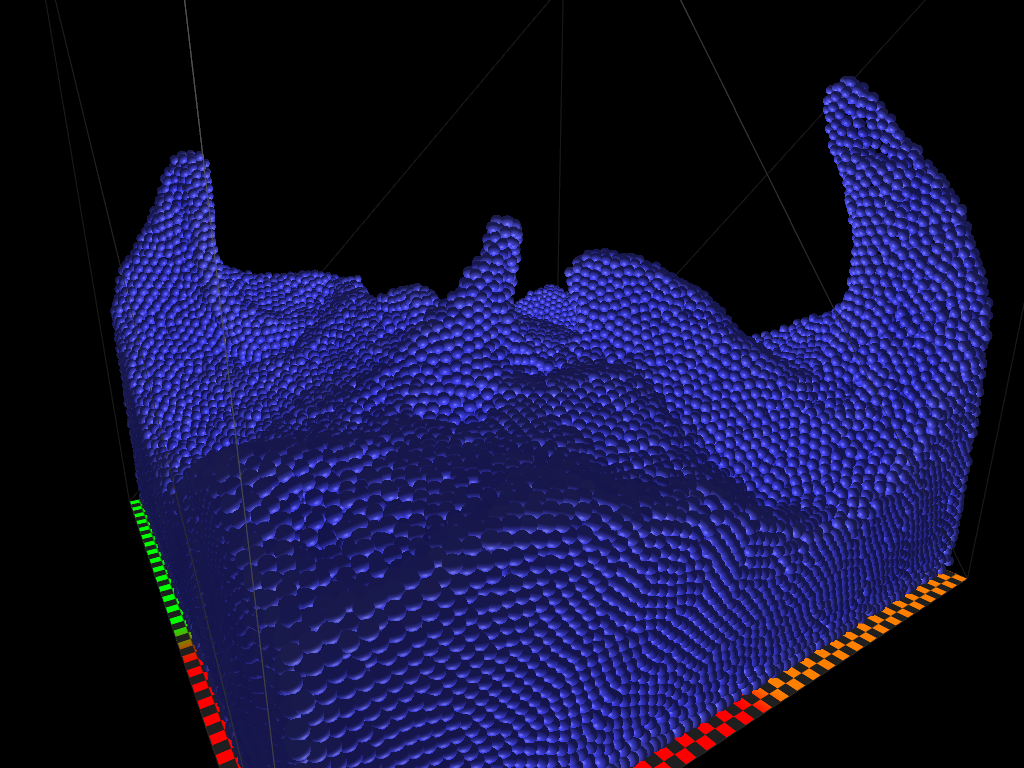
\includegraphics[width=0.9\textwidth]{img/55296_edit.png}
  \caption{}
\end{subfigure}%
\\
\begin{subfigure}{.9\textwidth}
  \centering
  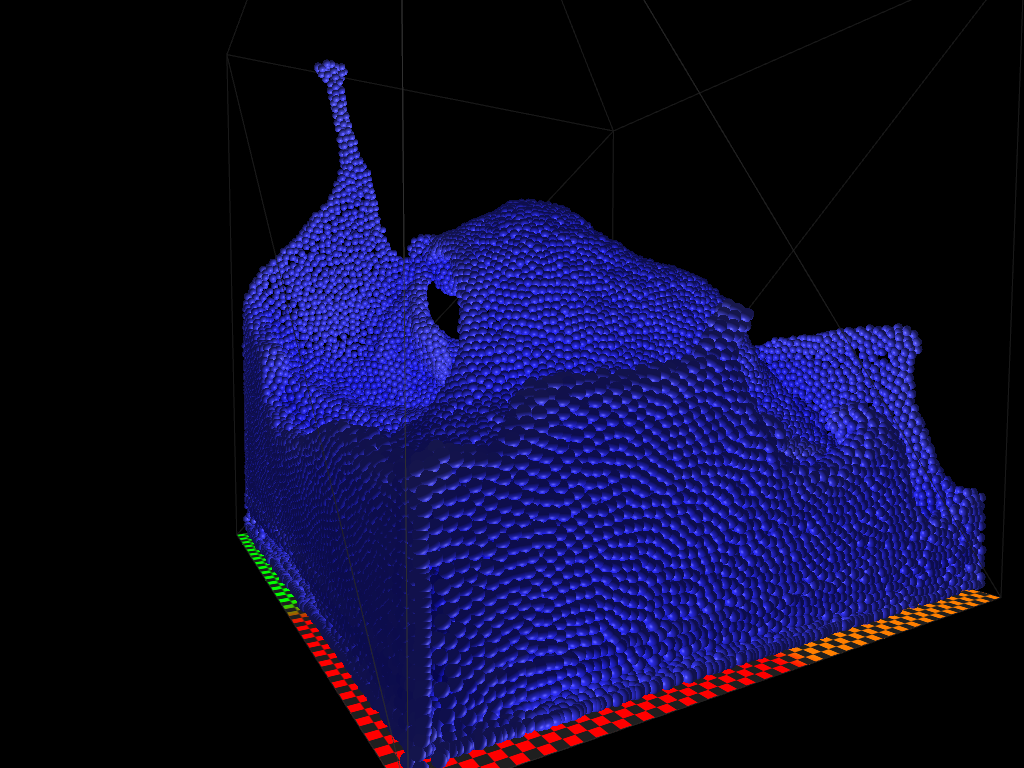
\includegraphics[width=0.9\textwidth]{img/3Nieghbours_55size.png}
  \caption{}
\end{subfigure}%

\caption{Two snapshots of our simulation, where (b) involves neighbouring particles at a larger distance resulting in slightly more curls than (a), due to the vorticity.}
\label{fig:result}
\end{figure}

\begin{figure}[H]
\hspace*{-2.1cm}
  \label{fig:graph}
  \centering
  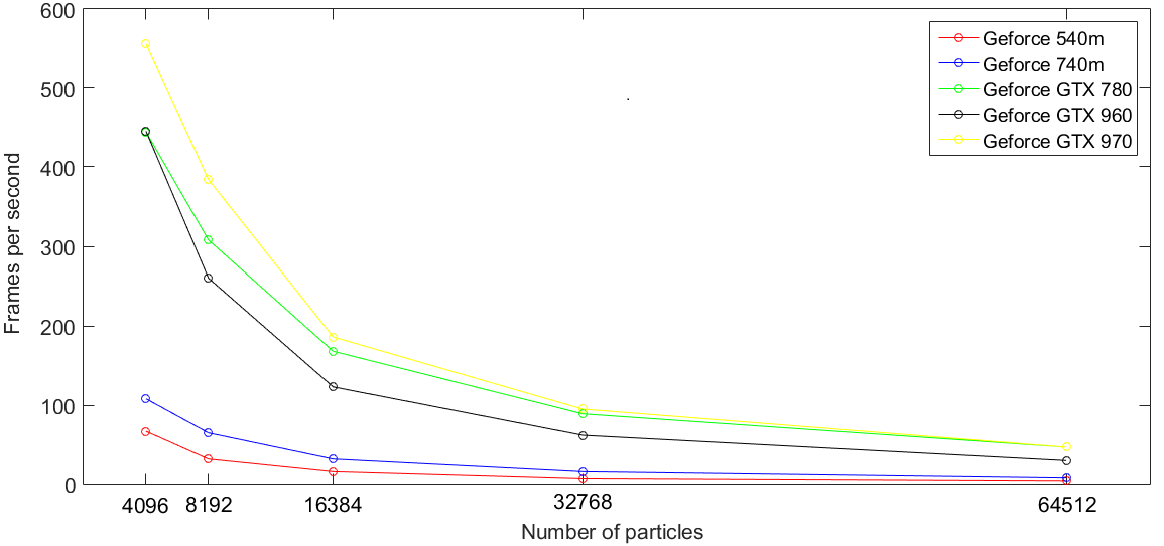
\includegraphics[scale=0.5]{img/graph.png}
  \caption{Performance when varying the number of particles on different GPUs}
\end{figure}


